\documentclass[12pt]{article}
%packages
\usepackage{amsmath, amsthm, amssymb}
\usepackage{graphicx}
\usepackage{enumerate}
\usepackage[utf8]{inputenc}
% \usepackage[spaced=0]{diffcoeff}
\usepackage[italic=true]{derivative}
\usepackage{tcolorbox}
\usepackage{physics2}
\usephysicsmodule{ab, braket}
\usepackage{siunitx}
\usepackage{fancyhdr}
\usepackage[margin=1in]{geometry}
\usepackage{tikz}
\usepackage{pgfplots} % for the axis environment
% \usepackage{fullpage}

%environments
\newtheorem*{question}{Q}
\newtheorem*{prop}{Proposition}

\newenvironment{quest}[1]
{\vspace{0.3cm}\noindent\textbf{Q(#1)}\em}{\vspace{0.3cm}}

\newenvironment*{Remark}{\noindent\textbf{Remarks}\begin{enumerate}}{\end{enumerate}\vspace{1em}\noindent}


\usepackage{hyperref}
\hypersetup{
    colorlinks=true,
    linkcolor=blue,
    filecolor=magenta,      
    urlcolor=cyan,
    pdftitle={Overleaf Example},
    pdfpagemode=FullScreen,
}


%commands
\newcommand{\e}{\varepsilon}
\newcommand{\R}{\mathbb{R}}
\newcommand{\Z}{\mathbb{Z}}
\newcommand{\N}{\mathbb{N}}
\newcommand{\C}{\mathbb{C}}
\newcommand{\Q}{\mathbb{Q}}


\newcommand{\grad}{\vec \nabla}
\newcommand{\LL}{\mathcal{L}}
\newcommand{\vphi}{\varphi}
\newcommand{\p}{\partial}



\newcommand{\eq}{\Leftrightarrow}
\newcommand{\clm}{\textbf{Claim }}
\newcommand{\rmks}{\noindent\textbf{Remarks}}

\newcommand{\levi}{\mathfrak{E}}


\makeatletter
     \newcommand\vb{\@ifstar\boldsymbol\mathbf}
     \newcommand\va[1]{\@ifstar{\vec{#1}}{\vec{\mathrm{#1}}}}
     \newcommand\vu[1]{%
       \@ifstar{\hat{{#1}}}{\hat{{#1}}}}
    % \renewcommand*{\vec}[][default]{def}
\makeatother


\newcommand{\ev}[1]{\langle{#1}\rangle}
\newcommand{\vecp}[1]{\vec{#1}\:'}
%\renewcommand\qedsymbol{QED}

%%%%%%%%%%%%%%%%%%%%%%
% Set up header/footer
\pagestyle{fancy}
\fancyhead[LO,L]{Vishwanath Wimalasena}
\setlength{\headheight}{14.5pt}
\fancyfoot[LO,L]{}
\fancyfoot[CO,C]{\thepage}
\fancyfoot[RO,R]{}
\renewcommand{\headrulewidth}{0.5pt}
\renewcommand{\footrulewidth}{0.4pt}
\renewcommand{\headrulewidth}{0.5pt}
%%%%%%%%%%%%%%%%%%%%%%



\tcbuselibrary{theorems}
\tcbuselibrary{breakable}
\tcbuselibrary{skins}

%environments
\newtheorem{theorem}{Theorem}[section]
\newtheorem{proposition}{Proposition}[section]
\newtheorem{definition}{Definition}[section]
\newtheorem{lemma}{Lemma}[section]
\newtheorem{lem}{Lemma}
\newtheorem*{ex}{Exercise}

\theoremstyle{definition}
\newtheorem*{sol}{Sol}

\newtcbtheorem[number within=section]{cthm}{Theorem}%
{colback=green!8!white, colframe=green!40!black,fonttitle=\bfseries, fontupper=\itshape}{mainthm}

\newtcbtheorem[number within=section]{cexercise}{Exercise}%
{colback=green!8!white, colframe=green!40!black,fonttitle=\bfseries, fontupper=\itshape}{mainthm}

\newtcbtheorem[number within=section]{cclaim}{Claim}%
{colback=green!8!white,colframe=green!40!black,fonttitle=\bfseries, fontupper=\itshape}{claim}

\tcolorboxenvironment{sol}{breakable, enhanced, left=5mm,
    before skip=10pt, after skip=10pt, frame  hidden,colback=green!6!white,
    borderline west={1pt}{0pt}{green!60!black}}

\tcolorboxenvironment{lem}{
    enhanced jigsaw,colback=green!8!white, colframe=green!40!black,breakable,before skip=10pt,after skip=10pt }

\tcolorboxenvironment{proof}{% `proof' from `amsthm' 
    blanker,breakable,left=5mm,
    before skip=10pt,after skip=10pt,
    borderline west={1pt}{0pt}{green!60!black}}

% \newtcolorbox{ansbox}{tcbox raise base, leftrule=0pt, arc=0pt, rightrule=0pt,toprule=0mm,bottomrule=0mm, colback=green!8!white, colframe=green!20!black}

% \newtcolorbox{background}[1][]{enhanced,
%     colback=green!5!white,colframe=green!40!black,
%     colbacktitle=green!40!black,fonttitle=\bfseries,
%     frame hidden,
%     title=Background,
%     boxrule=0pt,
%     titlerule style=green!70!black, #1}

\tcolorboxenvironment{ex}{enhanced jigsaw, colback=green!8!white, colframe=green!40!black,breakable,before skip=10pt,after skip=10pt}

\tcolorboxenvironment{question}{% `proof' from `amsthm' 
    blanker,colback=green,breakable,left=5mm,
    before skip=10pt,after skip=10pt,
    borderline west={1mm}{0pt}{green!40!black}}

% \tcbset{one-sided-color/.style={
%         breakable,
%         enhanced,
%         boxrule=0pt,
%         frame hidden,
%         borderline ={1pt}{0pt}{#1},
%         colback=#1!10,
%         coltitle=#1!200,
%         after title={\ },
%         attach title  to upper,
%     }
% }

\newtcolorbox{q}{one-sided-color=green!60!black, title=\textbf{Q}}

\newtcolorbox{outline}[1]{one-sided-color=blue!70!black, title=\textbf{#1}}

% \newtcolorbox{ans}{breakable,
%         enhanced,
%         boxrule=0pt,
%         frame hidden,
%         borderline west={1pt}{0pt}{green!70!black},
%         % borderline south={1pt}{0pt}{green!70!black},
%         % after title={\ },
%         % attach title  to upper,
%         top=1pt,
%         % boxsep=1pt,
%         colback=white,
%         coltitle=green!70!black!200}


% \newtcolorbox{q2}{breakable,
%         enhanced,
%         boxrule=0pt,
%         frame hidden,
%         borderline west={1pt}{0pt}{green!70!black},
%         colback=green!70!black!10, after title={Q}}

% \newtcolorbox{exc}[1]{one-sided-color=green!70!black, title=\textbf{(#1)}}
\definecolor{bordercolor}{rgb}{0.13,0.57,0.07}
\definecolor{boxcolor}{rgb}{0.28,0.69,0.28}

\newtcolorbox{exc}[1]{
        breakable,
        enhanced,
        frame hidden,
        borderline ={1pt}{0pt}{bordercolor},
        colback=boxcolor!10,
        coltitle=bordercolor,
        after title={\ },
        attach title  to upper,
        title=\textbf{Exercise #1},
        }

\newtcolorbox{ans}{
    breakable,
    enhanced,
    boxrule=0pt,
    frame hidden,
    borderline west={1pt}{0pt}{bordercolor},
    top=0pt,
    colback=white,
    coltitle=bordercolor,
    }
% \newcommand{\exc}[1]{\begin{exc}#1\end{exc}}

\fancyhead[CO,C]{\textbf{PHYS606}}
\fancyhead[RO,R]{PSET 1}

\newcommand{\HH}{\mathcal{H}}
\newcommand{\norm}[1]{||#1||}
\newcommand{\pv}{\mathcal{P}}
\newcommand{\ubra}[1]{\langle #1 \vert}
\newcommand{\uket}[1]{\vert #1 \rangle}
\newcommand{\ubraket}[2]{\langle #1 \vert #2 \rangle}


\begin{document}
\begin{exc}{1a}
\end{exc}
\begin{ans}
    Set $\ket{1}$ to have 0 energy. Move to rotating frame, valid if $\delta(t)$ assumed to vary slowly compared to ..., apply RWA to get 
    \[\HH = -\hbar \delta(t) \ketbra{2}{2} - \hbar\ab(\frac \Omega 2 \ketbra{2}{1} + \frac{\Omega}{2} \ketbra{1}{2}) \simeq -\hbar \begin{pmatrix}
        0 & \Omega /2\\
        \Omega/2 & \delta(t)
    \end{pmatrix}\]
    Eigenvalues $E$ of matrix given by 
    \[-E(\delta(t) - E) - \frac{\Omega^2}{4} = 0 \implies E= -\frac \hbar 2 (\delta \pm \underbrace{\sqrt{\delta^2 + \Omega^2}}_{:= \Omega_R})\]
    With eigenvectors satisfying
    \begin{align*}
        E\begin{pmatrix}
          v_1 \\ v_2  
        \end{pmatrix} = \begin{pmatrix}
            -\hbar \Omega/2 v_2 \\ 
            -\hbar \Omega/2 v_1 - \hbar \delta(t) v_2
        \end{pmatrix}
    \end{align*}
    This gives us $v_2 = - \frac{E}{\hbar}v_1$.
    Let $E_{A}, E_B$ refer to the $+, -$ eigenstates respectively. Then, our corresponding eigenstates are 
    \begin{align*}
        E_A &= -\frac \hbar 2 (\delta + \Omega_R), \qquad \ket{A(t)} = \frac1{N_A}(\Omega \ket{1} + (\delta + \Omega_R)\ket 2) \\
        E_B &= -\frac \hbar 2 (\delta - \Omega_R), \qquad \ket{B(t)} = \frac1{N_B}(\Omega\ket{1} + (\delta - \Omega_R)\ket2)
        % = = \ket{1} - \frac 2\hbar E_A\ket 2
        %  = \Omega \ket{1} -\frac 2\hbar E_A \ket 2
    \end{align*}
    with the normalizations given by 
    \begin{align*}
        N_A &= \sqrt{\Omega^2 + (\delta + \Omega_R)^2}, \qquad N_B = \sqrt{\Omega^2 + (\delta - \Omega_R)^2} 
        % = \sqrt{\Omega^2 + \frac{4E_A^2}{\hbar^2}}
        % = \sqrt{\Omega^2 + \frac{4E_A^2}{\hbar^2}}
    \end{align*}
    As $\delta \to \infty$, $\Omega_R \to \delta$ and we get 
    \begin{align*}
        E_A \to -\hbar \delta, \quad \ket{A(t)} \to \ket{2}        \\
        E_B \to 0, \quad \ket{B(t)} \to \ket{1}
    \end{align*}
    As $\delta \to -\infty$, $\Omega_R \to -\delta$ and
    \begin{align*}
        E_A \to 0, \qquad \ket{A(t)} \to \ket{1} \\
        E_B \to -\hbar \delta, \qquad \ket{B(t)} \to \ket{2}
    \end{align*}
    which is expected as $|\delta| \gg \Omega$ implies a weak driving field. In the limit $\Omega = 0$, our hamiltonian is diagonal with $\ket{1}$ corresponding to eigenenergy 0 and $\ket{2}$ to $-\hbar \delta = \hbar(\omega - \nu)$ (the energy of $\ket{2}$ in the non-rotating frame shifted down by $\nu$). See the Figure below for reference. 
\end{ans}
\begin{figure}[h!]
    \centering 
    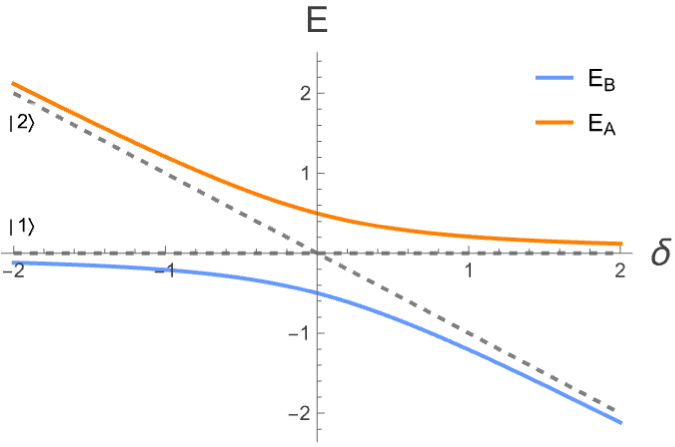
\includegraphics[width=0.6\textwidth]{1b_detuning.png}
    \caption{Energy of dressed states against detuning for 2 level system in Problem 1 with dashed lines indicating energies for zero field eigenstates of 0 and $-\hbar \delta$}
\end{figure}

\begin{exc}{1b}
\end{exc}
\begin{ans}
Remark: $i\hbar \uket{\dot A(t)} \neq H\ket{A(t)}$ because $A(t)$ is an instantaneous eigenvector of $H$ and the time dependence is due only to $\delta(t)$.


With $\ket{\psi(t)} = a(t)\ket{A(t)} + b(t)\ket{B(t)}$, we get
\begin{equation*}
    i\hbar \uket{\dot \psi(t)} = i\hbar\ab(\dot a(t) \ket{A(t)} + a(t) \uket{\dot A(t)} + \dot b(t) \ket{B(t)} + b(t) \uket{\dot B(t)})
\end{equation*}
and 
\begin{equation*}
    H\ket{\psi(t)} = a(t)E_A\ket{A(t)} + b(t) E_B\ket{B(t)}
\end{equation*}
Thus, applying $\bra{A(t)}$ and $\bra{B(t)}$ to both sides of the schrodinger equation gives
\begin{align*}
    i\hbar \dot a  + i \hbar b \ubraket{A}{\dot B} &= a E_A  \\
    i\hbar a \ubraket{B}{\dot A} + i \hbar \dot b &= bE_B 
\end{align*}
where $\braket{A}{A} = \braket{B}{B} = 1$ due to normalization and $\ubraket{A}{\dot B} = \ubraket{B}{\dot A} = 0$ by Lemma \ref{lemma:1b_linalg_results}. 

% From 1a, we have that 
% \[\ket{\dot A} = -\frac{2}{\hbar}\dot E_b \ket{2} = \dot\delta\ket{2}, \qquad \ket{\dot B} = -\frac{2}{\hbar}\dot E_A\ket{2} = \dot \delta \ket{2}\]
% We have the inner products 
% \begin{align*}
%     \braket{A}{\dot B} &= \dot \delta(\delta - \Omega_R) \\
%     \braket{B}{\dot A} &= \dot \delta (\delta + \Omega_R)
% \end{align*}
% To determine $\ubraket{A}{\dot A}$, we note that 
% \[N_A = \braket{A}{A} \implies \odv{N_A}{t} = \braket{\dot A}{A} + \braket{A}{\dot A} = 2\braket{A}{\dot A}\]
% We calculate 
% \begin{align*}
%     \odv{N_A}{t} = \frac{4}{\hbar^2} 2E_B\dot E_B = \frac{4}{\hbar^2} 2E_b \cdot (-\frac\hbar 2 \dot\delta) = -\frac{4E_b \dot \delta}{\hbar} \implies \braket{A}{\dot A} = -\frac{2E_B\dot\delta}{\hbar} 
% \end{align*}
% Similarly, 
% \[\braket{B}{\dot B} = -\frac{2E_A\dot \delta}{\hbar}\]
% the last step holds since $\ket{A}$ is imbedded in a real vector space spanned by $\ket{1},\ket{2}$.

Thus, it remains to calculate $\ubraket{A}{\dot B}$. We leave this to mathematica (see the accompanying notebook). Our result is  
\[\ubraket{A}{\dot B} = \frac{\dot\delta\Omega}{2(\delta^2 + \Omega^2)} = -\ubraket{B}{\dot A}\]
Plugging in these inner products gives us the EOMs 
\begin{align*}
    i \hbar \dot a  + i \hbar b  \frac{\dot\delta\Omega}{2(\delta^2 + \Omega^2)}  &= aE_A  \\
    -i\hbar a  \frac{\dot\delta\Omega}{2(\delta^2 + \Omega^2)} + i\hbar \dot b &= bE_B
\end{align*}
Simplifying gives us 
\begin{align}
    \label{eqn:1a_EOMS_for_a}
    \dot a &= - \frac{iE_A}\hbar a  - \frac{\dot\delta\Omega}{2(\delta^2 + \Omega^2)}  b\\ 
    \label{eqn:1a_EOMS_for_b}
    \dot b &= - \frac{iE_B}{\hbar} b + \frac{\dot\delta\Omega}{2(\delta^2 + \Omega^2)} a
\end{align}
In the adiabatic limit where $\delta$ changes very slowly, $\dot \delta \approx 0$ and we get
\begin{align*}
     \dot a &= - \frac{iE_A}\hbar a, \qquad \dot b = -\frac{iE_B}{\hbar} b
\end{align*}
this implies that our state $\ket{\psi(t)}$ just picks up phase factors on the basis states $\ket{A(t)}, \ket{B(t)}$ and does not mix these states. We can then, for example, follow $\ket{A(t)}$ from $\delta \ll 0$ to $\delta \gg 0$ to traverse from $\ket{2} \to \ket{1}$. 
\end{ans}

\begin{lem}
    \label{lemma:1b_linalg_results}
     We claim the following results
    \begin{enumerate}
        \item If $\ket{A(t)}$ is normalized and exists in a real vector space, then $\ubraket{A}{\dot A} = 0$
        \item Eigenvectors of Hermitian matrix are orthogonal 
    \end{enumerate}
\end{lem}
\begin{proof}[Proof of 1.]
    By assumption, $\braket{A(t)}{A(t)} = 1$, so 
    \[0 = \odv{}{t}\braket{A(t)}{A(t)} = \ubraket{\dot A}{A} + \ubraket{A}{\dot A} = \ubraket{A}{\dot A}^* + \ubraket{A}{\dot A} = 2\ubraket{A}{\dot A}\]
\end{proof}
\begin{proof}[Proof of 2.]
    Let $v_i$ be eigenvectors of hermitian operator, $A$, with different eigenvalues, $\lambda_i$. Then 
\[\braket[3]{v_i}{A}{v_j} = \lambda_i \braket{v_i}{v_j} = \lambda_j \braket{v_i}{v_j} \implies (\lambda_i - \lambda_j)\braket{v_i}{v_j} = 0\]
\end{proof}

\begin{exc}{1c}

\end{exc}
\begin{ans}
    We have $a(t) = a(0)e^{-i E_At/\hbar}$ and $b(t) = b(0) e^{-i E_Bt/\hbar}$. For $\ket{\psi(0)} = \ket 1 = a(0)\ket{A(0)} + b(0) \ket{B(0)} \approx a(0)\ket{2} + b(0) \ket{1}$, if we begin very negatively detuned. This gives $a(0) = 0$ and $b(0) = 1$. Thus, $a(t) = 0$ and $b(t) = e^{-iE_bt/\hbar}$. Hence, 
    \[\ket{\psi(t)} = e^{-iE_Bt/\hbar}\ket{B(t)}\]
    Thus, if we adiabatically change the detuning from negative to positive, $\ket{B(t)}$ goes from state $\ket 1 \to \ket 2$ as shown in 1a. By this method, we can take the inital population in state 1 to state 2. 
\end{ans}


\begin{exc}{1d}

\end{exc}
\begin{ans}
    We want equations \ref{eqn:1a_EOMS_for_a} and \ref{eqn:1a_EOMS_for_b} to be uncoupled. The coupling term is $\dot \delta \Omega/(2 (\delta^2 + \Omega^2))$. The other relevant physical equantity is the energy \emph{difference} $|E_A - E_B|/\hbar$. For adiabatic passage, we impose that
    \[\frac{\dot \delta \Omega}{2 (\delta^2 + \Omega^2)} \ll \frac1\hbar(E_A - E_B) = \frac12(\delta + \Omega_R - (\delta - \Omega_R)) = \Omega_R\]
    Thus,
    \[\dot \delta \ll \frac{2\Omega_R(\delta^2 + \Omega^2)}{\Omega}\]
    The lower limit of this expression occurs when $\delta = 0$ and $\Omega_R \to \Omega$. For the inequality to hold at all $\delta$, we require 
    \[\dot \delta \ll \frac{2\Omega(\Omega^2)}{\Omega} = 2\Omega^2\]
    as desired.

    For a resonant $\pi$ pulse, we use a pulse duration $\tau$ defined by $\Omega T\tau = \pi \implies \tau = \pi/\Omega$. In comparison, if $\odv{\delta}{t} \ll 2\Omega^2$, then we have 
    \[\delta(T) - \delta(0) \ll 2\Omega^2 T \implies T \gg \frac{\delta(T) - \delta(0)}{2\Omega^2} > \frac{2\Omega}{\Omega^2} = \frac1\Omega \approx \frac{\pi}{\Omega} = \tau\]
    where population inversion requires $|\delta| \gg \Omega$ and if $\delta(0) < 0$, then $\delta(T) - \delta(0) > 2\Omega$. We conclude that adiabatic passage thus requires much longer times than resonant pulses.
\end{ans}


\begin{exc}{1e}

\end{exc}
\begin{ans}
\textbf{Advantages}
\begin{enumerate}
    \item No need to stay on resonance during entire measurement period
    \item Detuning is easily controlled by frequency of driving field.
\end{enumerate}

\textbf{Disadvantages}
\begin{enumerate}
    \item Takes longer than pulses 
    \item Pulsed measurement schemes common in other fields like magnetic resonance. More literature/infrastructure to borrow from 
\end{enumerate}
\end{ans}


\newpage 
\begin{exc}{2a}

\end{exc}
\begin{ans}
    We work in the rotating frame with energies shifted down by $\nu$ so that $\ket{2}$ has energy $\hbar(\omega_{12} - \nu) = -\hbar\delta$ and $\ket{3}$ has energy $\hbar((\omega_{12} + \Delta \omega) - \nu) = \hbar(\Delta \omega - \delta)$. Then, our hamiltonian in the rotating frame with the RWA takes the form 
    \begin{align*}
        \HH = -\hbar \begin{pmatrix}
            0 &  \Omega/2  &  \Omega/2 \\ 
             \Omega/2 & \delta & 0 \\ 
             \Omega/2 & 0 & -(\Delta \omega - \delta)
        \end{pmatrix}
    \end{align*}
    as expressed in the basis $\{\ket 1, \ket 2, \ket 3\}$. We also took $\Omega$ to be real by appropriate choice of phase factor for the basis states. Writing an arbitrary state as $\ket{\psi(t)} = c_1(t) \ket 1 + c_2(t) \ket 2 + c_3(t) \ket 3$, the schrodinger equation gives us $i\hbar \odv{}{t}\ket{\psi(t)} = \HH \ket{\psi(t)}$ so that 
    \begin{align*}
        \dot c_1(t) \ket 1 + \dot c_2(t) \ket 2 + \dot c_3(t) \ket 3 
        &= ic_1 \frac \Omega2 \ket 2 + ic_1 \frac \Omega2 \ket 3 + ic_2 \frac \Omega2\ket 1 \\
        & \qquad + ic_2\delta \ket 2 + ic_3\frac \Omega2\ket 1 - ic_3(\Delta \omega - \delta)\ket 3
    \end{align*}
    Orthogonality gives us the equations 
    \begin{align*}
        \dot c_1 &= i\frac \Omega2c_2  + i\frac \Omega2c_3\\
        \dot c_2 &= i\frac \Omega2 c_1 + i\delta c_2 \\ 
        \dot c_3 &= i\frac \Omega2 c_1 - i(\Delta \omega - \delta)c_3
    \end{align*}
\end{ans}

\begin{exc}{2b}
    
\end{exc}
\begin{ans}
    We use adiabatic expansion to deal with $c_3$. Our first order expansion, $\dot c_3^{(1)}$ comes from setting $\dot c_3 = 0$, so that  
    \[0 = \dot c_3 = i\frac \Omega 2 c_1 - i(\Delta \omega - \delta) c_3^{(1)} \implies c_3^{(1)} = \frac \Omega{2(\Delta \omega - \delta)} c_1\]
    Our second order expansion $c_3^{(2)}$ satisfies 
    \begin{align*}
        \dot c_3^{(1)} &= i\frac \Omega 2 c_1 - i(\Delta \omega - \delta)c_3^{(2)}\\ 
        \frac{\Omega}{2(\Delta \omega - \delta)}\dot c_1 &= i\frac \Omega 2 c_1 - i(\Delta \omega - \delta)c_3^{(2)}\\
        \frac{\Omega}{2(\Delta \omega - \delta)}\ab(i\frac \Omega2c_2  + i\frac \Omega2c_3^{(2)}) &= i\frac \Omega 2 c_1 - i(\Delta \omega - \delta)c_3^{(2)}
    \end{align*}
    From this, we get 
    \begin{align*}
        \Omega^2c_2  + \Omega^2c_3^{(2)} &= 2\Omega(\Delta \omega - \delta) c_1 - 4(\Delta \omega - \delta)^2c_3^{(2)} \\ 
        c_3^{(2)}( \Omega^2 + 4(\Delta \omega - \delta)^2) &= 2\Omega(\Delta \omega - \delta) c_1 - \Omega^2 c_2 \\ 
        c_3^{(2)} &= \frac{2\Omega(\Delta \omega - \delta) c_1 - \Omega^2 c_2 }{\Omega^2 + 4(\Delta \omega - \delta)^2}
    \end{align*}

    Plugging back into our original equation for $\dot c_1$, we get 
    \begin{align*}
        \dot c_1 
        &=  i\frac{\Omega}2 c_2 + i\frac \Omega 2 \ab(\frac{2\Omega(\Delta \omega - \delta) c_1 - \Omega^2 c_2 }{\Omega^2 + 4(\Delta \omega - \delta)^2}) \\ 
        &= \frac{i\Omega}2\ab(1  - \frac{\Omega^2}{\Omega^2 + 4(\Delta \omega - \delta)^2})c_2 + \frac{i\Omega^2(\Delta \omega - \delta)}{\Omega^2 + 4(\Delta \omega -\delta)^2}c_1
    \end{align*}
    Since we are expanding to second order, $\Omega^2/(\Delta \omega - \delta)^2 \ll 1 \implies \Omega^2 \ll (\Delta \omega - \delta)^2$. With this in mind, we get 
    \begin{align*}
        \dot c_1 
        &\approx \frac{i\Omega}2\ab(1  - \frac{\Omega^2}{4(\Delta \omega - \delta)^2})c_2 + \frac{i\Omega^2(\Delta \omega - \delta)}{4(\Delta \omega -\delta)^2}c_1\\
        &= \frac{i\Omega}2\ab(1  - \frac{\Omega^2}{4(\Delta \omega - \delta)^2})c_2 + \frac{i\Omega^2}{4(\Delta \omega -\delta)}c_1
    \end{align*}
\end{ans}

\begin{exc}{2c}

\end{exc}
\begin{ans}
    We use our first order adiabatic expansion, $c_3{(1)} = \frac{\Omega}{2(\Delta \omega - \delta)}c_1$ from part (b) to get the system 
    \begin{align*}
        \dot c_1 &= \frac{i\Omega}2 c_2 + \frac{i\Omega^2}{4(\Delta \omega - \delta)}c_1 \\ 
       \dot c_2 &= \frac{i\Omega}2c_1 + i\delta c_2
    \end{align*}
    If the effects of state $\ket 3$ were ignored ($\Delta \omega \to \infty)$, we would have Rabi oscillations at frequency $\Omega/2$ during resonance. To achieve oscillations, we require $\ddot c_i \propto - c_i$ for $i = 1,2$. Differentiating $c_1$ twice, we see that
    \begin{align*}
        \ddot c_1 &= \frac{i\Omega}2\ab(\frac{i\Omega}2c_1 + i\delta c_2)  + \frac{i\Omega^2}{4(\Delta \omega - \delta)} \ab(\frac{i\Omega}2  c_2 + \frac{i\Omega^2}{4(\Delta \omega - \delta)}c_1)\\
        &= -\ab(\frac{\Omega^2}4 + \frac{\Omega^4}{16(\Delta \omega - \delta)^2}) c_1 + \frac{i\Omega}{2}\ab(i\delta + \frac{i\Omega^2}{4(\Delta \omega - \delta)})c_2
    \end{align*}
    Thus, we get the desired form for $\ddot c_1$ iff 
    \[\delta = -\frac{\Omega^2}{4(\Delta \omega - \delta)} \implies \delta = 2\Delta \omega \pm \sqrt{4\Delta\omega^2 + \Omega^2}\] 
    Take the $+$ solution since the problem assumes $\delta  = \nu - \omega_{12} > 0$.


    If such $\delta$ is chosen, then the effect of state 3 is to induce a phase shift so that the oscillation frequency goes from $\frac \Omega 2 \to \sqrt{\frac{\Omega^2}4 + \delta^2}$. Otherwise, for relatively weak driving fields or large detuning, our system looks like $\dot c_1 = \Omega^2/(4(\delta \omega - \delta)) c_1$ and $\dot c_2 = -i\delta c_2$, so that state 3 causes an energy shift by $\delta = \Omega^2/(4(\delta \omega - \delta))$ to state 1. This looks like an AC stark shift.
\end{ans}

\begin{exc}{2d}

\end{exc}
\begin{ans}
Using our answer for part (3) that the effect of state 3 looks like a stark shift of $\Omega^2/(4(\Delta \omega - \delta))$ for general $\delta$, we see that this will cause phase evolution of the states as $e^{-i \Omega^2t/(4\Delta \omega - \delta)}$. To minimize this effect, we require 
\[\frac{\Omega^2}{4(\Delta \omega - \delta)}t \ll 1 \implies t \ll \frac{4(\Delta \omega - \delta)}{\Omega^2}\]

For $\delta = 0$, we get 
\[t \ll \frac{4\Delta \omega}{\Omega^2}\]
The rabi oscillations between states occur at frequency $\Omega/2$, so a full rotation occurs when $T\Omega/2 = 2\pi \implies T = 4\pi/\Omega$. Thus, the number of full rotations we can perform before decoherence is 
\[\#\textrm{(Full Rotations)} = \frac{t}{T} = \frac{4\Delta \omega / \Omega^2}{4\pi/\Omega} = \frac{\Delta \omega}{\pi\Omega}\]
In the spin resonance example, we get 
\begin{align*}
    t \ll \frac{4(100 - 0)}{10^2}\frac1{\unit{MHz}} = 4 \unit{\micro s}
\end{align*}
and the number of rotations is
\[\frac{100}{10\pi } = \frac{10}{\pi} \approx 3.1\]
\end{ans}
\newpage 
\begin{exc}{3a}

\end{exc}
\begin{ans}
    We expand $\ket{\psi(t)}$ in terms of the bound state $\ket{b}$ and continuum states, indexed by $\ket{k}$, as 
    \begin{align*}
        \ket{\psi(t)} = b(t)\ket{b} + \sum_{k = -\infty}^\infty c_k(t) \ket{k}
    \end{align*}
    Schrödinger's equation gives us 
    \begin{align*}
        i\hbar \dot b = \bra{b} \HH \ket{\psi(t)} &= -\hbar \sum_{k = -\infty}^\infty f^*g c_k \\ 
        i\hbar \dot c_k  = \bra{k}\HH \ket{\psi(t)} &= \hbar (\omega_k - \nu)c_k -\hbar fg b
    \end{align*}
    Set $\delta_k = \nu - \omega_k$. Thus, we get the system 
    \begin{align*}
        \dot b &= i\sum f^*g c_k \\ 
        \dot c_k &= i\delta_k c_k + ifgb
    \end{align*}
    Formally integrating $c_k$ gives us 
    \[c_k(t) = ig\int_0^t e^{i\delta_k(t - \tau)}f(\tau)b(\tau)d\tau + c_k(0)e^{i\delta_kt}\]
    We assume that the $\ket{\psi(0)} = \ket{b}$ so $c_k(0) = 0$.
    Then, we get 
    \begin{align*}
        \dot b = -g^2 \sum_{k = -\infty}^\infty f^*(t)\int_0^t e^{i\delta_k(t - \tau)}f(\tau)b(\tau)d\tau 
    \end{align*}
    We are given that $f$ is slowly varying so we approximate $f(\tau)\approx f(t)$. We use the Markovian assumption to do the same for $b(\tau) \approx b(t)$. Then, we get 
    \begin{align*}
        \dot b &\approx -g^2 |f(t)|^2 b(t) \sum_{k = -\infty}^{\infty}\int_0^t e^{i\delta_k(t - \tau)}d\tau \\ 
        &\approx  -g^2 |f(t)|^2 b(t) \sum_{k = -\infty}^{\infty}(\pi \delta(\delta_k) + i\pv\frac1{\delta_k})
    \end{align*}
    Now we separate variables to get 
    \begin{align*}
        \frac{db}{b} = - dtg^2|f(t)|^2 \sum_{k = -\infty}^{\infty}(\pi \delta(\delta_k) + i\pv\frac1{\delta_k})
    \end{align*}
    Integrating and using the initial condition $b(0) = 1 \implies \ln(b(0)) = 0$, we get
    \[\ln(b(t)) = \int_0^t d\tau g^2|f(\tau)|^2\sum_{k = -\infty}^\infty  (\pi \delta(\delta_k) + i\pv\frac1{\delta_k})\]
    Thus, 
    \[
    b(t) = \exp\ab[\sum_{k = -\infty}^\infty  (\pi \delta(\delta_k) + i\pv\frac1{\delta_k}) \int_0^t d\tau g^2|f(\tau)|^2]
    \]
\end{ans}


\begin{exc}{3b}
\end{exc}
\begin{ans}
    The outgoing state is spanned by the $\ket k$ states, so 
    \[\uket{\psi^{\textrm{out}}} = \sum_{k = -\infty}^\infty c_k(t)\ket{k}\]
    The real-space wavefunction is given by 
    \begin{align*}
        \psi^{\textrm{out}}(x, t) = \ubraket{x}{\psi^{\textrm{out}}} = \sum_{k = -\infty}^\infty c_k(t) \braket{x}{k} = \sum_{k = -\infty}^\infty c_k(t)e^{ikx}
    \end{align*}
    With density of states $\odv{N}{k} = \rho$, we can take $N = \sum_k \to \int \rho dk$, so that
    \begin{align*}
        \psi^{\textrm{out}}(x, t) 
        &= \int_{-\infty}^\infty \rho c_k(t) e^{ikx}dk\\
        &= ig \int_{-\infty}^\infty  \rho e^{ikx} \int_0^t e^{i\delta_k(t - \tau)}f(\tau)b(\tau)d\tau dk \\ 
        &= ig \rho \int_0^t f(\tau)b(\tau) \int_{-\infty}^\infty e^{ikx}e^{i \delta_k(t - \tau)}dk d\tau \\ 
         &= ig \rho \int_0^t f(\tau)b(\tau) \int_{-\infty}^\infty e^{ikx}e^{i(\nu - v_0|k|)(t - \tau)}dk d\tau \\ 
         &= ig \rho \int_0^t f(\tau)b(\tau) e^{i\nu(t - \tau)}\int_{-\infty}^\infty e^{ikx}e^{iv_0|k|(t - \tau)}dk d\tau   \\ 
         &= i 2\pi g \rho \int_0^t f(\tau)b(\tau) e^{i\nu(t - \tau)}\ab[\delta(x - v_0(\tau - t)) + \delta(x + v_0(\tau + t))]d\tau 
    \end{align*}
    We calculate the inner integral as 
    \begin{align*}
        I &= \int_{-\infty}^\infty e^{ikx}e^{iv_0|k|(t - \tau)}dk\\ 
        &= \int_{-\infty}^0 e^{ikx}e^{-iv_0k(t - \tau)}dk + \int_{0}^\infty e^{ikx}e^{iv_0k(t - \tau)}dk \\
        &= \int_{-\infty}^0 e^{ik(x - v_0(t - \tau))}dk + \int_{0}^\infty e^{ik(x + v_0(t - \tau)}dk
    \end{align*}
    With $x' = x \pm v_0(t - \tau)$, we recognize these integrals as Fourier transforms of the function $f(k) = 1$, . Hence, we get $\mathcal F\{1\} = 2\pi \delta(x')$. Thus, 
    \begin{align*}
        I = 2\pi\delta(x - v_0(t - \tau)) + 2\pi\delta(x + v_0(t - \tau))
    \end{align*}
    Substituting back into our original wavefunction, we find 
    \begin{align*}
         \psi^{\textrm{out}}(x, t) 
         &= ig \rho \int_0^t f(\tau)b(\tau) e^{i\nu(t - \tau)}\ab[2\pi\delta(x - v_0(t - \tau)) + 2\pi\delta(x + v_0(t - \tau))]d\tau  \\
         &= i2\pi g \rho\bigg(\Theta(x)\Theta(t - x/v_0)f(t - x/v_0)b(t - x/v_0)e^{i\nu x/v_0} \\ 
         & \qquad +  \Theta(-x)\Theta(t + x/v_0)f(t + x/v_0)b(t + x/v_0)e^{-i\nu x/v_0}\bigg)
    \end{align*}
\end{ans}
\end{document}


